\textbf{Reliability Relevance Evaluation}
Given this theoretical foundation, the challenge is how to evaluate the reliability relevance of edges in  a given uncertain graph efficiently ($\mathcal{E}RR-$eval). 
For each edge $e$, we need to measure the reliability difference over $\mathcal{G}_{e}$ and $\mathcal{G}_{\bar{e}}$. 
This evaluation involves the two-terminal reliability detection problem, which is known to be NP-complete~\cite{MOBall}.   


A baseline algorithm for $\mathcal{E}RR-$eval is to use the
Monte Carlo sampling. More precisely, we sample $N$ possible
worlds of the input uncertain graph, where $N$ is large enough (around $1,000$) to guarantee high approximation accuracy. 
Over each sampled possible world (Say $G$), we carry out a connected-component computation algorithm to count 
the number of connected pairs $cc(G)$. Then, the count on the original uncertain graph $cc(\mathcal{G})$ can be estimated by taking the average over the sampled deterministic graphs. 

\begin{theorem}
	The complexity of the baseline $\mathcal{E}RR-$eval algorithm is $\mathcal{O} (|E| \cdot  N \alpha(|V|) |E| )$ where $\alpha$ is the inverse Ackermann function.  
\end{theorem}

{\bf Proof sketch} The time complexity of the connected component detection algorithm based on the union-find method is $\mathcal{O}(\alpha(|V|) |E|)$~\cite{Wredman:1989:CPC:73007.73040}. Consequently, computing the $\mathcal{E}RR$ for an edge over the $N$ possible worlds takes time $\mathcal{O}(N \alpha(|V|) |E|)$, and the total time complexity for all the edges is $\mathcal{O} (|E| \cdot  N \alpha(|V|) |E|)$. 


\begin{figure}
	\centering
    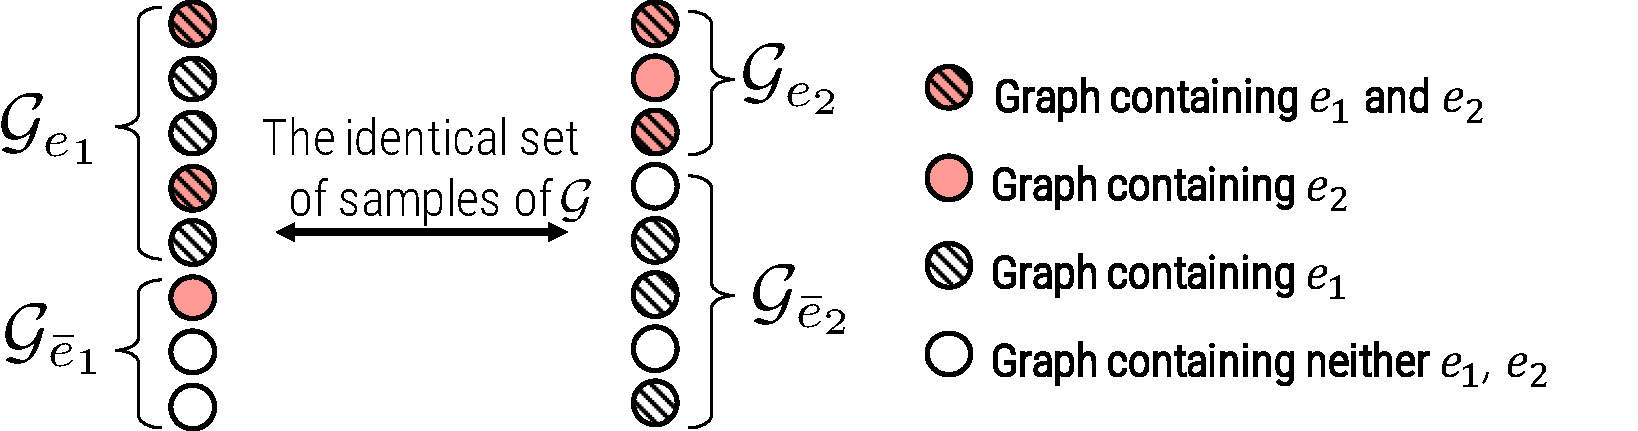
\includegraphics[width=1\linewidth]{ill/rrEval.pdf}
    \vspace{-1em}
    \caption{\small Reused sampling estimator for $\mathcal{E}RR$ }
    \label{fig:rrEval}
%     \vspace{-1em}
\end{figure}
Obviously, the baseline algorithm is inefficient when the input uncertain graph is very large (it is quadratic in the number of edges). Here, we present a efficient algorithm for $\mathcal{E}RR$ evaluation in Algorithm~\ref{alg:RReval}. Its basic idea is to re-use the connected components detection result of samples as illustrated in~\ref{fig:rrEval}. For each edge $e$, we group the sampled possible worlds according to the edge existence (Line 4-6), then get the sampled average of $cc$ for each group as accurate approximation of $cc(\mathcal{G}_{e})$ and $cc(\mathcal{G}_{\bar{e}})$. By this way, we bring the the evaluation of edge reliability relevance to the realm.  

\begin{theorem}
	The time complexity of Algorithm\ref{alg:RReval} $\mathcal{E}RR-$val is $\mathcal{O}(N \alpha(|V|) |E|)$ where $N$ is the number of samples.
\end{theorem}



\begin{algorithm}[!tb]
{\scriptsize
    \begin{algorithmic}[1]
       \item[] {\textbf{Input:} ~$\mathcal{G}=(V,E,\mathit{p})$, $N$ is the number of sampled graphs;~}
       \item[] {\textbf{Output:} ~$\mathcal{E}RR$ Reliability relevance of edges in $\mathcal{G}$}
    \STATE {$CC_{e} \leftarrow  \mathbf{0} $, $CC_{\bar{e}} \leftarrow \mathbf{0}$}
    \FOR{i=1 \TO N }
    \STATE {$G \leftarrow $  A deterministic sampled instance}
    \STATE {$Ind(G)$ is edge existence of sampled graph $\mathcal{G}$}
    \STATE {$cc(G) \leftarrow $ the number of connected pairs of $G$}
    \STATE {$CC_{e}+=Ind(G) \cdot cc(G)$,$CC_{\bar{e}}+=(\mathbf{1}-Ind(G)) \cdot cc(G)$ }
    \ENDFOR
    \STATE{$\mathcal{E}RR= CC_{e}/\mathit{p} - CC_{\bar{e}}/{\mathbf{1}-\mathit{p}}$}
         \caption{Edge Reliability Relevance Evaluation}
        \label{alg:RReval}
    \end{algorithmic}
    }
\end{algorithm}
